\documentclass[relqm.tex]{subfiles}

\begin{document}
\part{Gauge Theories}
\chapter{}
\section{Plan}
\begin{itemize}
    \item Lectures 1-2: Introduction and Motivation, Intro to Group theory $\to$ Lie groups (continoues symmetries).
        \begin{itemize}
            \item Why group theory? Gauge theories are quantum field theories with an emphasis on symmetry, as gauge theories have gauge symmetries. Mathematically, symmetries are described by group theory. 
        \end{itemize}
    \item Lecture 3: Different types of symmetries - global and local (gauge) symmetries. 
    \item Lecture 4: From these gauge symmetries, we will construct Abelian, and non-Abelian gauge field theories. 
    \item By the end of the course, we will learn about the Higgs mechanism and Spontaneous Symmetry Breaking, and ultimately reach the full Standard Model of Particle Physics.
\end{itemize}
The Standard Model is a gauge field theory of SU(3)$\times$SU(2)$\times$U(1) - this is the gauge group of the Standard Model. 
\begin{itemize}
    \item SU(3) is the gauge theory of strong interactions (QCD).
    \item SU(2)$\times$U(1) is the gauge theory of the unified electroweak interactions.
\end{itemize}

\section{Introduction to Group Theory}
Groups are needed in order to describe and define symmetry transformations. 
So what is a group?

There are four properties that define a group:
\begin{enumerate}
    \item \textbf{Closure} under group multiplication. 
        \begin{align}
            g_1\cdot g_2 = g_3 \in G,\; \forall g_1,g_2 \in G
        \end{align}
        So group multiplication is confined to within the bounds of the group.
    \item \textbf{Associativity} of group multiplication. 
        \begin{align}
            g_1\cdot(g_2\cdot g_3) &= (g_1\cdot g_2)\cdot g_3,\; \forall g_1,g_2,g_3 \in G
        \end{align}
    \item \textbf{Identity element}. 
        \begin{align}
            \exists\, e \in G\,:\, e\cdot g = g\cdot e = g,\; \forall g \in G
        \end{align}
    \item \textbf{Inverse element}.
        \begin{align}
             \exists\, g^{-1} \in G\,:\, g^{-1}\cdot g = g\cdot g^{-1} = e,\; \forall g \in G
        \end{align}
\end{enumerate}

Now some notes:
\begin{itemize}
    \item The group is called \textbf{Abelian} iff
        \begin{align}
            g_1\cdot g_2 = g_2\cdot g_1,\; g_1,g_2 \in G
        \end{align}
        This is equivalent to being called commutative, from $[g_1,g_2]=0$.
    \item Then it holds that we have \textbf{non-Abelian} groups, where
        \begin{align}
            g_1\cdot g_2 \neq g_2\cdot g_1
        \end{align}
        This is non-commutative, from $[g_1,g_2]\neq0$.
\end{itemize}
Matrix multiplication (of square matrices) is an example of a non-Abelian group multiplication.

\subsection{Important Examples}
\begin{itemize}
    \item SU(N) is a group of unitary $N\times N$ matrices, with $\text{det}=1$. For SU(N), N is for $N\times N$ matrices, and the U says it is unitary. 
        Unitary is defined by
        \begin{align}
            SU(N) \ni U\,:\, U^\dagger\cdot U = U\cdot U^\dagger = \mathbb{I}_{N\times N},~ U^\dagger = (U^*)^T
        \end{align}
        where $U^\dagger$ is called Hermitian conjugation. 
        The S then defines the group as "Special", which means $\text{det}(U) = 1$.\\
        Let's check these group properties. 
        \begin{enumerate}
            \item Matrix multiplication:
                \begin{align}
                    U_1 &\in SU(N):~ U_1^\dagger U_1 = \mathbb{I} \\
                    U_2 &\in SU(N):~ U_2^\dagger U_2 = \mathbb{I} \\
                    (U_1U_2)^\dagger U_1U_2 &= U_2^\dagger \underbrace{U^\dagger_1 U_1}_{\mathbb{I}}U_2 = U^\dagger_2 U_2 = \mathbb{I} \\
                    \text{det}(U_1U_2) &= \text{det}(U_1)\cdot\text{det}(U_2) = 1
                \end{align}
                So we have \textbf{closure.}
            \item Associativity is satisfied by the definition of matrix multiplication.
            \item Unit matrix:
                \begin{align}
                    e &= \mathbb{I}_{N\times N} 
                \end{align}
            \item The inverse matrix element:
                \begin{align}
                    U^{-1} &= U^\dagger
                \end{align}
        \end{enumerate}
        So we have a group that holds all the properties, a very important group at that. \\
        Consider some general $U \in SU(N)$. 
        How many real independent parameters (real degrees of freedom) does $U$ have?
        An $N\times N$ complex matrix will have $2N^2$ real degrees of freedom. 
        Now if we require unitarity, $U^\dagger = U$, there are $N^2$ constraints on the degrees of freedom, so now we are left with only $N^2$ degrees of freedom by this requirement. 
        Now if we impose that $\text{det}U = 1$, which is a single condition, we are left with $N^2-1$ real degrees of freedom. 
    \item U(1) is a group of unitary $1\times1$ matrices, so $U^\dagger U = 1$. 
        \begin{align}
            \forall U \in U(1)\,:\, U = e^{i\alpha},\; \alpha \in \R
        \end{align}
        Note we cannot require that the $\text{det}U=1$, otherwise we collapse down to a single value of this group, where $\alpha=0$.
        We do not really need to check the group properties of U(1) as they are completely trivial.
    \item SO(N) is a group of $N\times N$ real-valued matrices which are orthogonal:
        \begin{align}
            \forall O \in SO(N)\,:\, O^T\cdot O = O\cdot O^T = \mathbb{I}
        \end{align}
        So N is for $N\times N$, O is for orthogonal, and S again for $\text{det}=1$.\\
        SO(N) matrices are \emph{proper} (we do not do parity transformations of $x\to -x$) rotations in the $\R^N$ (N-dimensional real vector space).
        It is again trivial to find the four group properties fully satisfied for SO(N), so these are groups again.
        \begin{align}
            SO(2) \ni O = \begin{pmatrix} \cos\theta & \sin\theta \\ -\sin\theta & \cos\theta\end{pmatrix}
        \end{align}
        We can see that for SO(2), we have one real parameter in $\theta\in\R,0\leq\theta\leq2\pi$.
\end{itemize}

\chapter{}
Continuing last time, SO(2) is isomorphic to U(1):
\begin{align}
    SO(2):~ O &= \begin{pmatrix}\cos\theta & \sin\theta \\ -\sin\theta & \cos\theta\end{pmatrix} & U(1):~ U &= e^{i\theta} = \cos\theta + i\sin\theta
\end{align}
So both these groups depend only on the value of $\theta$, and knowing any matrix in one of these groups allows us to construct the corresponding matrix in the other.

\section{Group Theory Continued}
\subsection{Direct Products of Groups}
Consider a group $G \ni \{g_1,g_2,\dots\}$, and another group $H \ni \{h_1,h_2,\dots\}$.
We can define a product group from these, $G\times H$, which is also a group. 
The definition of this direct product is by construction.
If we consider a matrix element of matrix $g \in G,\, g_{ij}$, and similarly for in $H$ we consider the matrix element $h_{\alpha\beta}, h \in H$.
Now we construct an object
\begin{align}
    g_{ij}\cdot h_{\alpha\beta} &\equiv (gh)_{i\alpha;j\beta} \\
    G\times H &= \{g_{ij}\cdot h_{\alpha\beta}\}
\end{align}
Let us consider the example of $U(1)\times SU(2)$, where this direct product is equal to $U(2)$, which is a untary group, but the determinant is not $=1$, but $\text{det}=e^{i2\alpha}$, where $\alpha$ was the parameter of $U(1)$.

An important example to keep in mind is the Gauge Field Theory of the Standard Model: $SU(3)\times SU(2)\times U(1)$.

\subsection{Simple vs Non-simple Groups}
\textbf{A simple group} is defined as a group that cannot be written as a direct product of smaller groups, i.e. cannot be decomposed.
A group U(N) is not simple, as
\begin{align}
    U(N) &\approx U(1)\times SU(N),
\end{align}
where SU(N) and U(1) are both trivially simple groups. 

\subsection{Representations of Groups}
We can describe group in two equivalent ways:
\begin{itemize}
    \item A group is some formal mathematical structure - it is some set of elements which satisfies the four definitions of the group and some precise descriptions of what we mean by that.
    \item \textbf{The Fundamental Represenation of the Group} - we can derive a group via an explicit matrix representation, e.g. SU(N) are $N\times N$ complex matrices such that $U^\dagger U=1 = UU^\dagger$ and $\text{det}U=1$.
\end{itemize}
Each group can have many different representations; the fundamental representation is what we used for its definitions.
A group SU(N) in the fundamental representation is given by the $N\times N$ matrices.
These matrices act on some N-dimensional complex vector space described by a N-vector.
\begin{align}
    \begin{pmatrix} \bullet & \bullet & \bullet \\ \bullet & \bullet & \bullet \\ \bullet & \bullet & \bullet \end{pmatrix} \cdot \begin{pmatrix} \bullet \\ \bullet \\ \bullet\end{pmatrix}
\end{align}
An N-vector, $x_i$, is transforming in the fundamental representation of SU(N).

We can also construct a tensor representation,
\begin{align}
    x_i &= \begin{pmatrix} x_1\\ x_2\\x_N\end{pmatrix};y_j = \begin{pmatrix}y_1\\y_2\\y_N\end{pmatrix} \in \C^N:~ x_iy_j = \text{rank-2 tensor, in SU(N)} \\
    \sum_k & \underbrace{U_{ik}}_{\text{SU(N) matrix}}\underbrace{x_k}_{\text{vector}} = \underbrace{x'_i}_{\text{\shortstack{transformed\\ vector}}} \text{ fund. rep.} \\
    \sum_{j'}\sum_{i'} & U_{ii'}U_{jj'}(x_{i'}y_{j'}) = (xy)_{ij}
\end{align}
These rank-two tensor representations can be decomposed into a singlet $\oplus$ traceless symmetric tensor $\oplus$ anti-symmetric tensor representations.
These representations which cannot be reduced any further are called \textbf{irreducible representations.}
So the fundamental representation of any group is irreducible, while rank-two tensor representation is reducible, as said above.

A group element in some general representation can be written as some matrix which can be brought into some block diagonal form, where off-diagonal elements are all zero, where each minimal block along the diagonal is an irreducible representation (irrep) of the group.

\chapter{}
\section{Lie Groups}
For a Lie group, $G$, with an element of this group, $a(\alpha^1,\dots,\alpha^k)$, $a$ depends continuously on parameters $\alpha^1,\dots,\alpha^k$. 
Elements of Lie groups can be represented by
\begin{align}
    a &= e^{-i\sum_{a=1}^k T^a\alpha^a}.
\end{align}
Here, the $\alpha$s are our free parameters, and $T^a$ are the generators of the Lie group, i.e. these are given matrices.
\begin{align}
    \alpha^i=0\; \forall\, i \leq k,\; a = e^0 = \mathbb{I}
\end{align}
We can consider $\alpha^1,\dots,\alpha^k\ll1$ (infinitesimal),
\begin{align}
    a &= e^{-i\sum_{a=1}^k T^a\alpha^a} = \mathbb{I} - i\sum_a T^a\alpha^a + \mathcal{O}(\alpha^2) \\
    T^a &= i\frac{\p a}{\p\alpha^a}\bigg|_{\alpha^a=0}
\end{align}
For example, if $G=SU(2)\ni U_{2\times2}$ (in the fundamental representation):
\begin{align}
    T^b_{2\times2} &= i\frac{\p U_{2\times2}}{\p\alpha^b}
\end{align}
Now back to the general case of a Lie group (\textit{from now on, the sum over repeated indices is assumed}),
\begin{align}
    G \ni a &= \exp\left(-iT^a\alpha_a\right) \\
    T^a &= i\frac{\p a}{\p\alpha^a}\bigg|_{\alpha^a=0}
\end{align}
This will find our generators for the Lie group, but these generators will not commute:
\begin{align}
    [T^a,T^b] &= if^{abc}T^c
\end{align}
This is not an elephant, but another generator with some prefactor, where the $f^{abc}$ is the structure constant of the Lie group. 
Following from the definition of the commutator relation, $f^{abc}$ is completely anti-symmetric around its three indices.

\textbf{Any given Lie group is defined by this relation in Eq (3.8).}
Essentially, the explicit form of the structure constants is what defines any given Lie group as distinct.
From this relation, we can find the set of all generators, $\{T^a\}^k_{a=1}$, which will allow us to write down all elements of our Lie group, $a\in G$ through Eq (3.1).

\subsection{Notations}
Sometimes in the notes, we may use 
\begin{align}
    a &= e^{i\theta^a X_a},~ \theta^a = -\alpha^a,~ X^a = T^a \\
    c^{abc} &=  f^{abc}
\end{align}

\section{Some Simple Lie Groups}
\subsection{U(1) Group}
The simplest example we'll have is U(1) $\ni a$: here, we have $T=1$, and the number of generators is also 1.
        \begin{align}
            a &= e^{-i\alpha\cdot1},~ T=1 \\
            [T,T] &= [1,1] = 0 \implies f^{abc} = 0
        \end{align}
        For all Abelian Lie groups, the commutators are zero (by definition).

\subsection{SU(2) Group}
SU(2) $\ni U$:
\begin{align}
    U &= e^{-i\alpha^a T_a}
\end{align}
So we want to know:
\begin{itemize}
    \item How many $T^a$s are there, i.e. $k$? And what are the generators of SU(2) in the fundamental representation? \\
        We will start by choosing the fundamental representation, where we have $2\times2$ complex matrices with $U^\dagger U = \mathbb{I}$ and $\text{det}U = 1$.
        \begin{align}
            U &= \exp\left(-i\sum_{a=1}^3 \alpha^a\frac{\sigma^a}{2}\right)
        \end{align}
        So we have three real parameters in $\alpha^a$ and the generators, $\frac{\sigma^a}{2}$ are the Pauli matrices (over 2). 
        Is this right?
        Well Pauli matrices are Hermitian, and they provide us with a complete basis of $2\times2$ Hermitian matrices (-1, as it excludes the unit matrix).
        Let's consider the Hermitian conjugate of $U$ to check:
        \begin{align}
            U^\dagger &= \left[\exp\left(-i\alpha^a\frac{\sigma_a}{2}\right)\right]^\dagger = \exp\left(+i\alpha^a\frac{\sigma_a}{2}\right) = U^{-1}
        \end{align}
        So we have unitarity, and we can easily check the other group properties if needed.

        We have learned that the generators of SU(2) (in the fundamental representation) are 
        \begin{align}
            T^a &= \frac{\sigma^a}{2},~ a = \{1,2,3\}
        \end{align}
        This agrees with the argument of free parameters from last lecture where SU(N) has $N^2-1$ free parameters, which for SU(2) requires three free parameters, which we have in our three generators. 
        
        But why is it $\frac{\sigma}{2}$ and not $\sigma$? The $\frac12$ factor is due to normalisation, and depends on how we choose normalisation. 
        In the fundamental representation, we choose
        \begin{align}
            \text{Tr}(T^aT^b) &= \frac12 \delta^{ab},
        \end{align}
        and for $T^a = \frac{\sigma^a}{2}$, we fulfill this requirement.

    \item What is the Lie algebra of SU(2), i.e. $f^{abc}$?
        \begin{align}
            \left[\frac{\sigma^a}{2},\frac{\sigma^b}{2}\right] &= i\e^{abc}\frac{\sigma^c}{2}
        \end{align}
        We can check this directly using the defining properties of Pauli matrices, or just working it out by hand. 
        So our structure constants of SU(2) are $\e^{abc}$, and now we have our full Lie algebra for SU(2):
        \begin{align}
            [T^a,T^b] &= i\e^{abc}T^c
        \end{align}
    \item What about choosing in another representation than the fundamental one?\\
        We can choose any representation of SU(2), and we may get different descriptions of generators, but the Lie group is always defined by Eq (3.8), and for SU(2), $f^{abc} = \e^{abc}$ in any representation, but the simplest one will always be the fundamental one.
\end{itemize}

\chapter{}
\section{Symmetries: An Introduction}
Recall: The Fundamental representation of SU(N) has $T^a_{N\times N}$ acting on $\phi=\begin{pmatrix}x_1\\ n_N\end{pmatrix} \in \C$.
The conjugate to the fundamental representation takes $\phi^\dagger$ instead. 

In the adjoint representation, $(T^a)_{bc} = -if^{bca}$, a running from 1 to the number of generators, which is $N^2-1$ for SU(N).

Symmetries:\\
Let $\phi(x)$ be a field. 
Its Lagrangian is 
\begin{align}
    \La &= \frac{1}{\lambda}\p_\mu\phi\p^\mu\phi - \frac12m^2\phi^2 - \frac{\lambda}{4}\phi^4
\end{align}
for a simply-interacting real scalar field, $\phi(x)\in\R$.
The kinetic term is quadratic (bilinear) in the field, the interaction term is of a higher order. 
The kinetic terms yield propagators, here being $\frac{i}{p^2-m^2}$. 
The interaction terms yield vertices in the Feynman diagrams.

For a complex field,
\begin{align}
    \La &= (\p_\mu\phi^\dagger)(\p^\mu\phi) - m^2\phi^\dagger\phi - \frac{\lambda}{4!}(\phi^\dagger\phi)^2
\end{align}
For a general field, the action is
\begin{align}
    S = \int \La[\phi]\;d^4x
\end{align}
A transform of the fields which leaves the action invariant is called a symmetry. 
Additionally, a quantum theory must also leave the vacuum invariant. 

Symmetries can be discrete, e.g. $\phi(x)\to-\phi(x)$, or continuous, e.g. $\phi(x)\to e^{-i\alpha(x)}\phi(x),\alpha\in\R$.
The Lagrangian of a real scalar field is invariant under $\phi\to\phi(x)$, so the action is also invariant. 
Thus $\phi\to-\phi$ is a symmetry of this theory; for the complex scalar Lagrangian, $\phi\to e^{i\alpha}\phi$ is a symmetry. 
A continous symmetry can be local, depending on $x_N$, or global, being independent of $x_N$, i.e. if $\alpha$ in $e^{i\alpha}\phi$ is $\alpha(x)$ then it is local, and global if just $\alpha$.\\
Continuous transforms are described by Lie groups. 
Global continuous symmetries provide conserved quantities - this is the basis of Noether's theorem which states that for every generator of a global continuous system, there exists a conserved current $j^\nu(x)$ such that $\p^\nu j = 0$.
This is a Noether current. \\
For U(1), $\phi\to e^{-i\alpha}\phi$, which gives us the conserved electric charge, 
\begin{align}
    Q = \int j^\nu(x)\;d^3x,~ \frac{dQ}{dt} = 0
\end{align}

Noether's theorem does not necessarily hold for local symmetries. 
These are gauge symmetries. 
We consider a local U(1) transform, $\phi\to e^{-i\alpha(x)}\phi$, with the Dirac Lagrangian for free Dirac fermions, 
\begin{align}
    \La &= \bar{\psi}(i\gamma^\nu\p_\nu - m)\psi \\
    \La &\to \La + \bar{\psi}i\gamma^\nu\p_\nu(-i\alpha(x))\psi \text{ - not invariant}
\end{align}
To attain invariance, we add a gauge field $A$, that transforms as $A_\mu(x)\to A_\mu(x)+\frac{1}{e}\p_\mu\alpha(x)$, $e$ being the gauge coupling constant. 
We then replace the standard derivative with a covariant derivative of the form, 
\begin{align}
    D_\mu &= \p_\mu + ieA_\mu \\
    \La &= \bar{\psi}(i\gamma^\mu D_\mu - m)\psi
\end{align}
We now have a gauge invariant Lagrangian above which describes not only the propagatino of $\bar{\psi}$ and $\psi$, but it also includes the interaction between $A_\mu$ and $\psi$.
To give $A_\mu$, the photon propagation, we include a term $-\frac14 F^{\mu\nu}F_{\mu\nu}$ in the Lagrangian, where,
\begin{align}
    F^{\mu\nu} &= \p^\mu A^\nu - \p^\nu A^\mu,
\end{align}
which is plainly gauge invariant in the U(1) case. 
Thus, 
\begin{align}
    \La_{QED} &= \bar{\psi}(i\cancel{D} - m)\psi - \frac14 F^{\mu\nu}F_{\mu\nu}
\end{align}


\chapter{}
\section{QED}
The Lagrangian of QED:
\begin{align}
    \La = \bar{\psi}(i\gamma^\mu D_\mu - m)\psi - \frac14 F_{\mu\nu}F^{\mu\nu}
\end{align}
QED is a U(1) gauge invariance theory, with Dirac fermion fields $\psi,\bar{\psi}$, and the gauge field $A_\mu$, which is a vector field.
The Dirac fields describe $e^{\pm}$, and the gauge field describes the photons, $\gamma$.

If we consider just the gauge field part of QED:
\begin{align}
    \La[A_\mu] &= -\frac14 F^{\mu\nu}F_{\mu\nu}
\end{align} 
We can then begin to write down equations of motion from this, first considering the action.
\begin{align}
    \mathcal{S} &= \int \La[A_\mu]\,d^4x
\end{align}
We take the extremum of the action, where $\frac{\delta\mathcal{S}[A]}{\delta A_\nu}=0$, to find the Euler-Lagrange equations. 
\begin{align}
    \p_\mu \frac{\p\La[A]}{\p(\p_\mu A_\nu)} &= \frac{\p\La[A]}{\p A_\nu} = 0 \\
    \p_\mu F^{\mu\nu} &= 0
\end{align}
However, if we look at the full Lagrangian again and fully express $D_\mu = \p_\mu + ieA_\mu$, then Eq (5.5) is no longer equal to zero when fermions are present.
\begin{align}
    \p_\mu F^{\mu\nu} &= e\bar{\psi}\gamma^\nu\psi \equiv j^\nu
\end{align}
These are two of the Maxwell equations (out of four) for QED.
The other two Maxwell equations are trivial in QED, following from the Bianchi identity, 
\begin{align}
    \p_\lambda F_{\mu\nu} + \p_\mu F_{\nu\lambda} + \p_\nu F_{\lambda\mu} = 0.
\end{align}
This identity is automatically satisfied for $F_{\mu\nu} = \p_\mu A_\nu - \p_\nu A_\mu$.
So all four classical Maxwell equations can be written in QED as 
\begin{align}
    \frac{\p S}{\p A_\nu} = 0 &\implies \p_\mu F^{\mu\nu} = j^\nu \\
    \frac{\p S}{\p \bar{\psi}} = 0 &\implies (i\gamma^\mu D_\mu - m)\psi = 0  
\end{align}
Eq (5.9) is the Dirac equation with the field $A_\mu$ in the $D_\mu$ term. 

\subsection{How many degrees of freedom does the photon field have?}
Naively, it looks like it has four degrees of freedom, as we have $A_\nu, \nu = 0,1,2,3$. 
In reality, there are only two physical degrees of freedom of the photon.
Why is that?
$A_0$ field decouples $\to$ it is not a dynamical field as it does not have a kinetic term, i.e. $\frac12(\p_t A_0(x))^2$ is absent in the Lagrangian, but this term is required for any fieldto be kinetic as it would describe velocity.\\
We can always fix the gauge freedom by setting $A_0\equiv0$.
We can further set $\p_iA_i=0$ - this is the Coulomb gauge.
So we have two constraints from fixing the gauge, so two \emph{unphysical} degrees of freedom are removed, leaving us with $4-2=2$ physical degrees of freedom (assuming unbroken gauge invariance).
These 2 degrees of freedom of the photon are its 2 transverse polarisations. 

$A_\mu$ describes spin-1 fields (or particles), and we have the two gauges of $A_0 = 0$ and $\p_i A_i = 0 \implies p_i A_i = 0$, where $p_i$ is the three-momenta.
If we then choose momentum to be wholly along the z-coordinate, so $\vec{p}=(0,0,p)$, then $\vec{A} = (A_1,A_2,0)$, and then we see that we have two transverse polarisations along x and y, while the momentum transfer is all in z - this is the simplest choice for example but any physical orientation of $\vec{p}$ and $\vec{A}$ will lead to the same two transverse polarisations.

\subsection{What is allowed in QED?}
Again, we write down the QED Lagrangian:
\begin{align}
    \La_{QED} = &-\frac14 F^{\mu\nu}F_{\mu\nu} \text{ - propagator of the photon field $A_\mu$, quadratic in it} \nonumber \\
                &+ \bar{\psi}(i\gamma^\mu\p_\mu -m)\psi \text{ - free propagation of fermions} \nonumber \\
                &- e\bar{\psi}\gamma^\mu A_\mu\psi \text{ - 3 point vertex describing interactions}
\end{align}
$\La_{QED}$ is uniquely constructed from the requirement of gauge invariance. 
Can we add other gauge-invariant interactions?
Consider
\begin{align}
    \La &= F_{\mu\nu}F^{\nu\alpha}\tensor{F}{_\alpha^\mu}
\end{align}
For mass dimension, $[]$: we have
\begin{align}
    [A_\mu] &= 1 & [\phi] & = 1 & [\La] &= 4 \\
    [\psi] &= \frac32 & [\bar{\psi}] &= \frac32 & [\mathcal{S}] &= 0 
\end{align}
So we can see the mass dimension of the above $\La$ will be 6. 
We could add it to the QED Lagrangian with some pre-factor to get it to work?
\begin{align}
    \La &= \La_{QED} + \frac{1}{M^2}F_{\mu\nu}F^{\nu\alpha}\tensor{F}{_\alpha^\mu}
\end{align}
Any terms of $\La$ that have a coefficient of negative mass dimension in front are not UV-renormalisable, and any operators is $\La$ of mass dimension greater than 4 are not renormalisable. 

\subsection{What is UV Renormalisation?}
Any Quantum Field Theory which constains quantum corrections such as a tree level interaction, then one loop correction and up to higher loops, e.g.
\begin{equation}
    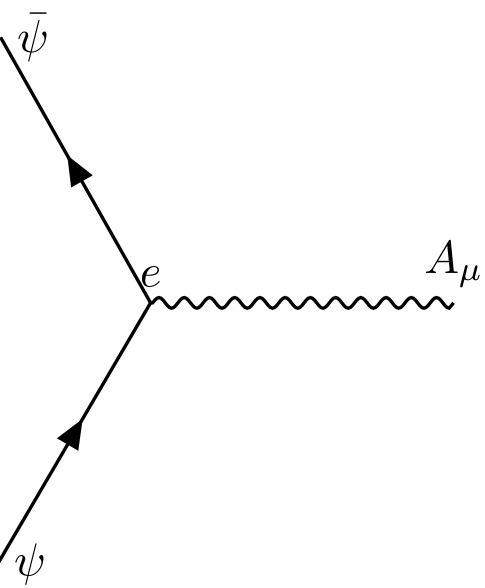
\includegraphics[valign=c,scale=0.2]{diagrams/renorm1.png} + 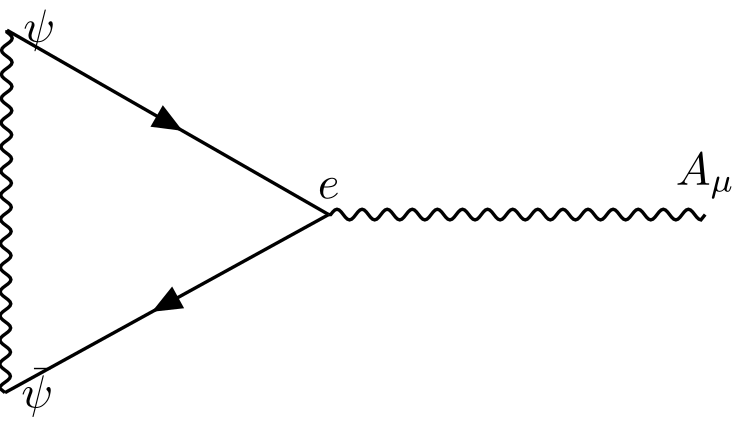
\includegraphics[valign=c,scale=0.2]{diagrams/norm2.png} + \dots
\end{equation}  
All loop-level corrections contain $\infty$ in the UV, so we need to have a prescription to remove this divergence.

\textbf{UV Renormalisation} is the prescription to remove UV divergences.

So now $\La_{QED}$ is completed and is shown that we cannot remove or add anything from/to it. 

\chapter{}
\section{Non-Abelian Gauge Invariance}
Start from a free Lagrangian for Dirac fermions
\begin{align}
    \La &= \bar{\psi}(i\gamma^\mu\p_\mu - m)\psi
\end{align}
$\psi(x)$ transform in the fundamental representation of a Lie group, G. 
Assume that G is a SU(N) group, so $\psi(x)$ is a column vector with $N$ rows 
$\bar{\psi}(x)$ will transform in the anti-fundamental representation, or conjugate to fundamental, as a row vector of $N$ columns.
This is invariant under global transformations. 
\begin{align}
    \psi(x) &\to U\psi(x),~ \bar{\psi}(x) \to \bar{\psi}(x)\,U^\dagger,~ U \in SU(N)
\end{align}
Here, U is not dependent on x, i.e. a global symmetry. 
The Lagrangian will be invariant. 
Upgrade this construction to $U(x)$, i.e. a gauge (local) symmetry. 
\begin{align}
    \psi(x)&\to U(x)\,\psi(x),\; \bar{\psi}(x) \to \bar{\psi}(x)\,U^\dagger(x),\; U(x) = e^{-i\alpha^a(x)T^a} \in SU(N) 
\end{align}
Here, $T^a$ are the generators of SU(N) in the fundamental representation. 
But here we will not see an invariant Lagrangian, so we must add something to the Lagrangian:
\begin{align}
    A_\mu(x) &\to U(x)(A_\mu(x)+i\p_\mu)U^\dagger(x)
\end{align}
In the fundamental representation, $U(x)$ is an $N\times N$ matrix, and $A_\mu$ must also be one for the equations to make sense - but this is still a single gauge field. 
The gauge field in matrix notation is then,
\begin{align}
    A_\mu(x) &= gT^aA_\mu^a(x).
\end{align}
$A_\mu^a$ is not a gauge field but a component gauge field, $a=0,\dots,N^2-1$; $g$ is the gauge coupling constant, i.e. a non-Abelian generalisation of $e$.

We can now form some trace identities (in the fundamental representation):
\begin{align}
    \text{Tr}[T^aT^b] &= \frac12\delta^{ab} & \text{Tr}[A_\mu T^a] &= \frac{g}{2}\sum_b A_\mu^b\delta^{ab} = \frac{g}{2}A_\mu^a & A_\mu^a &= \frac{2}{g}\text{Tr}[A_\mu T^a]
\end{align}
Now we can set out requirements to make our original $\La$ gauge invariant:
\begin{itemize}
    \item By transforming the derivative:
        \begin{align}
            \p_\mu &\to D_\mu = \p_\mu - iA_\mu
        \end{align}
        This is the \textbf{Covariant Derivative.}
    \item We must form a kinetic term for $A_\mu$s so that these are dynamical gauge fields
        \begin{align}
            \La_{kin} &= -\frac{1}{2g^2}\text{Tr}[F_{\mu\nu}F^{\mu\nu}]
        \end{align}
        $F_{\mu\nu}$ is the field strength:
        \begin{align}
            F_{\mu\nu} &= \p_\mu A_\nu - \p_\nu A_\mu - i[A_\mu,A_\nu]
        \end{align}
        This is almost the field strength that we had for QED, but we must add the final commutator term in order to make it transform as we are now in non-Abelian algebra. 
        $F_{\mu\nu}$ is the field strength in matrix notation, and can be written in component notation as well:
        \begin{align}
            F_{\mu\nu}(x) &= gT^aF^a_{\mu\nu}(x) & 
            F^a_{\mu\nu} &= \frac2g \text{Tr}[T^aF_{\mu\nu}] &
            F_{\mu\nu}^a &= \p_\mu A_\nu^a - \p_\nu A_\mu^a + gf^{abc}A_\mu^bA_\nu^c
        \end{align}
\end{itemize}
And our Lagrangian becomes
\begin{align}
    \La &= -\frac{1}{2g^2}\text{Tr}[F_{\mu\nu}F^{\mu\nu}] + \bar{\psi}(i\gamma^\mu D_\mu - m)\psi.
\end{align}
We still need to check if this is gauge invariant or not. 
How do $D_\mu\psi$ and $F_{\mu\nu}$ transform under gauge transforms?
\begin{align}
    F_{\mu\nu} &\to U\,F_{\mu\nu}\,U^\dagger & D_\mu\psi &\to U\,D_\mu\psi
\end{align}
So we see that $F_{\mu\nu}$ transforms in the adjoint representation, and $D_\mu\psi$ transforms as $\psi$.
How do we check these?
\begin{itemize}
    \item How to check for $F_{\mu\nu}$?
        \begin{align}
            F_{\mu\nu} &= \p_\mu A_\nu - \p_\nu A_\mu - i[A_\mu,A_\nu],\; A_{\mu,\nu} \to U(x)(A_{\mu,\nu} + i\p_{\mu,\nu})U^\dagger(x) \\
                       &\to U\,F_{\mu\nu}\,U^\dagger
        \end{align}
    \item How to check for $D_\mu\psi$?
        \begin{align}
            D_\mu\psi &= (\p_\mu + iA_\mu)\psi,\; \psi \to U(x)\psi(x),\; A_\mu \to U(x)(A_\mu+i\p_\mu)U^\dagger(x) \\
                      &\to U(x)D_\mu\psi
        \end{align}
\end{itemize}
We notice that that gauge transformation for $A_\mu \to (A_\mu(x)+\p_\mu)$ is really $A_\mu \to iD_\mu$.

So under gauge transformation, our Lagrangian transforms as:
\begin{align}
    \La &\to -\frac{1}{2g^2}\text{Tr}[UF_{\mu\nu}U^\dagger UF^{\mu\nu}U^\dagger] + \bar{\psi}U^\dagger(i\gamma^\mu UD_\mu\psi - mU\psi) \to \La
\end{align}
Hence, the Lagrangian is completely gauge invariant.

This is a universal prescription. 
For any Lagrangian with any matter fields (scalars, fermions, whatever else) that is invariant under global symmetry, performing the transformations
\begin{align}
    \p_\mu &\to D_\mu & \oplus \La_{kin} &= -\frac{1}{2g^2}\text{Tr}[F_{\mu\nu}F^{\mu\nu}]
\end{align}
will induce a gauge-invariant Lagrangian. 
Thus, we have constructed a non-Abelian gauge theory. 

Where does the kinetic pre-factor come from?
\begin{align}
    \La_{kin} &= -\frac{1}{2g^2}\text{Tr}[F_{\mu\nu}F^{\mu\nu}] = -\frac14F_{\mu\nu}F^{\mu\nu} \\
    F_{\mu\nu} &= gT^aF_{\mu\nu}^a,\; \text{Tr}[T^aT^b] = \frac12\delta^{ab}
\end{align}

This gauge theory is known as Yang-Mills theory, which is just meaning a non-Abelian theory. 
This theory is no longer free. 
It automatically contains interactions through the inclusion of $A_\mu$ which forms three-point vertices (interactions): between the fermions and gauge bosons, three gauge bosons; and four-point vertices between four gauge bosons.
This is not something we saw in QED, but nonetheless required for the Lagrangian to be physical at all. 

\chapter{}
We want to find a Lagrangian with terms with powers $>2$ of gauge fields, i.e. interactions of $A_\mu$s.
\begin{align}
    \La &= \dots - gf^{abc}\p_\mu A_\nu^aA^{\mu b}A^{\nu c} - \frac{g^2}{4}f^{abc}f^{ade}A_\mu^b A_\nu^c A^{\mu d}A^{\nu e} + \text{ nothing else}
\end{align}
From the first term, we can see that there interactions involving three-point vertices of gauge fields, 
\textit{doodle three-point vertex of three As} - $gf^{abc}p^\mu$
From the second, we find four-point vertices,
\textit{doodle four-point vertex of four As} - $gf^{abc}f^{ade}$
So interactions are automatically included, and there are no higher levels of gauge field interactions. 
Both the terms above had to appear in the Lagrangian as they come from $\frac{1}{2g^2}\text{Tr}[F_{\mu\nu}F^{\mu\nu}]$.\\
The relative coefficients between the three- and four-point vertices, and also between vertices with fermions, are fixed and uniquely determined by gauge invariance of the total Lagrangian. 
In a non-Abelian gauge theory, we cannot arbitrarily change the coupling constant $g$, e.g. if we coupled a matter field $\phi_1$ to $A_\mu$ with a coupling constant $g$, and try to couple some other matter field $\phi_2$ to $A_\mu$ with a coupling constant $\kappa g$, then $\kappa=1$.
If $\kappa\neq1$, then the $f^{abc}$s will be altered by this, which cannot be done as these define the group and will be constant. 
However, in an Abelian theory, we can couple different matter fields to gauge fields with $\kappa g$, where $\kappa$ is arbitrary. 

\section{Running Coupling Constants}
In a classical gauge theory, the coupling constant is a constant.
In a quantum gauge theory, it is no longer constant; instead, it depends on the energy scale at which we make observations. 
For a scattering experiment, at energy scale, $E = \sqrt{s}$, $s=(p_1+p_2)^2$.
\textit{doodle gluons going in and out, various diagrams at tree level and some loops}.
At tree level, processes are $\propto g^2$; at loop level, $\propto g^{2(1+\text{no. of loops})}$.
When we extract the value of $g^2$ from any such measurement, we will get $g^2(E)$.\\
We usually consider $g^2(p)$, where $p$ is a momentum or energy value characteristic for the experiment, e.g. can be $p=E_{COM}$, $p$ is either $\sqrt{s}$ or total transverse momentum (total momentum transfer).\\
Consider the coupling constant defined
\begin{align}
    \alpha(p) \equiv \frac{g^2(p)}{4\pi}.
\end{align}
In QED, we have $\alpha_{QED}=\frac{e^2}{4\pi}$.
In QCD, we have a SU(3) gauge theory with $N_f$ flavour of quarks (fermions), with a coupling constant (computed to 1 loop order),
\begin{align}
    \alpha_s(p) = \frac{g^2_{SU(3)}(p)}{4\pi} = \frac{2\pi}{b_0\log\frac{p}{\Lambda_{QCD}}}
\end{align}
Here, $\Lambda_{QCD}\approx300\,MeV$, $b_0=11-\frac23 N_f$. 

\chapter{}
For non-Abelian gauge theory, all matter fields couple to $A_\mu^a$ with the same gauge coupling $g$:
\begin{align}
    D_\mu &= \p_\mu - igA_\mu^aT^a.
\end{align}
For Abelian, this is not the case:
\begin{align}
    D_\mu &= \p_\mu + ieYA_\mu,
\end{align}
where we define $Y\equiv$ hypercharge - an arbitrary factor that can be different between matter fields.

In a non-Abelian theory, we can compute the coupling constant $\alpha(p)$, defined in Eq (7.2), as
\begin{align}
    \alpha(p) &= \frac{2\pi}{b_0\log\frac{p}{\Lambda}} + \text{ higher-order corrections.} \\
    \frac{2\pi}{\alpha(p)} &= b_0\log\left(\frac{p}{\Lambda}\right).
\end{align}
In an SU(N) gauge theory with $N_f$ flavours of Dirac fermions,
\begin{align}
    b_0 &= \frac{11}{3}N - \frac23 N_f.
\end{align}
Strong interactions in the Standard Model are described by QCD, the non-Abelian SU(3) gauge theory with $N_f=6$ quarks. 
In QCD, $b_0=7$, and what is important to note about that is that it is positively valued. 
$b_0$ is called the first coefficient of the $\beta$-function - the sign of the $\beta$-function and the sign of its first coefficient determines how the coupling constant runs. 
\begin{figure}[H]
    \centering
    \begin{tikzpicture}
        \draw[-Latex] (0,0) -- (5,0) node[anchor=north] {$\log p$};
        \draw[-Latex] (0,0) -- (0,2) node[anchor=east] {$\frac{1}{\alpha(p)}$};
        \draw (0.5,0) node[anchor=north] {$\Lambda$} -- (4.5,1.7);
    \end{tikzpicture}
\end{figure}
We can see at the scale of $\Lambda$, the coupling constant $\alpha$ becomes infinitely strong. 
More carefully:
\begin{itemize}
    \item Assume that our 1-loop approximation to $\alpha(p)$ is correct
    \item $p\to\Lambda \implies \frac{1}{\alpha}\to 0\implies\alpha\to\infty$, so we have an infinite strength interaction, which results in the confinement of quarks and gluons. 
\end{itemize}
This is non actually a full proof as the assumption is incorrect, but it does result in the real picture of confinement. \\
Similarly, $p\to\infty\implies\frac{1}{\alpha(p)}\to\infty\implies\alpha(p)\to0$, which results in \emph{asymptotic freedom}, i.e. at high energies, QCD interactions become irrelevant. 
The theory of QCD at high energies becomes free, or non-interacting. 

\chapter{}
\section{The Standard Model}
The Standard Model of particle physics is an SU(3)$_c\otimes$SU(2)$_L\otimes$U(1)$_Y$ gauge theory. 
SU(3) is the theory of strong interaction (QCD); and SU(2)$\otimes$U(1) is the GWS electroweak theory, where SU(2) describes what will become weak interactions, and U(1) describes what will become electromagnetic interactions (after spontaneous symmetry breaking).
\begin{itemize}
    \item $b_0>0$ for non-Abelian gauge theories (if $N_f <$ some critical number)
    \item $b_0<0$ for Abelian theories like U(1)
\end{itemize}
If we define three coupling constants: for QCD, $\alpha_S$; for weak, $\alpha_W$; and for QED, $\alpha_{EM}$.
\begin{figure}[H]
    \centering
    \begin{tikzpicture}
        \draw[-Latex] (0,0) -- (5,0) node[anchor=north] {$\log p$};
        \draw[-Latex] (0,0) -- (0,2) node[anchor=east] {$\frac{1}{\alpha(p)}$};
        \draw (0.5,0) node[anchor=north] {$\Lambda$} -- (4.5,1.7) node[anchor=west] {$\alpha_S$};
        \draw (0.2,0.3) -- (4.7,1.5) node[anchor=west] {$\alpha_W$};
        \draw[dashed] (0.8,0) -- (0.8,0.5);
        \draw (0.3,2) -- (4.8,0.2) node[anchor=west] {$\alpha_{EM}$};
    \end{tikzpicture}
\end{figure}
\begin{itemize}
    \item At the electroweak scale $\approx m_{W,Z,H}\approx100$ GeV, the weak force fails as its mediators are no longer present. 
    \item EM will hit zero in the graph at what is known as $\Lambda_{Landau}$ and freaks out from there.
    \item EM will fail like weak at the electron mass scale.
    \item All three coupling constants almost converge on a single point in the middle, but not quite. If they did, it would be indicative of a Grand Unified Theory (GUT) scale, i.e. SU(5)$_{GUT}\to$SU(3)$\otimes$SU(2)$\otimes$U(1). A single gauge theory of SU(5) would split into the three known groups at lower energy scales, below the GUT scale. 
        SU(5) is currently ruled out, but maybe SO(10)?
    \item $\alpha_W$ is small for all regions where the weak force manifests, so it can always be studied perturbatively.
    \item $\alpha_{\text{EM}}$ is fine in the IR regime (low energy) but then freaks out at higher energies, and cannot be studied perturbatively.
\end{itemize}

\section{QCD}
\begin{itemize}
    \item QCD has gauge group SU(3).
    \item What are the matter fields of QCD? Dirac fermions known as quarks, transforming in the fundamental representation of SU(3). 
        Quarks are in triplet states of colour, $q=\begin{pmatrix}q_1\\q_2\\q_3\end{pmatrix}$, where $q_i$ indicates the colour (1,2,3). 
        There are six flavours of quarks as well, so $q^f_i$ where $f$ is the flavour running $1\to6$ and $i$ is the colour running $1\to3$. 
        (Of course, each quark is also a Dirac spinor of 4 components.)
    \item In the infrared regime (low energy), $\alpha_S\to\infty$ which implies colour confinement.
    \item We cannot find free quarks or gluons in nature (in the IR range).
    \item What we can observe instead are colourless (SU(3) singlets) composite particles, i.e. mesons and baryons. 
    \item Mesons are quark-antiquark pairs: $\bar{q}_i^{f_1}q_i^{f_2}$, e.g. $\pi$-meson:
        \begin{align}
            \pi^0 &= \frac{\bar{u}u + \bar{d}d}{\sqrt{2}}, &
            \pi^- &= \bar{u}d, &
            \pi^+ &= \bar{d}u.
        \end{align}
        These are the lightest mesons using only the first generation of quarks. 
        $Q(u) = \frac23$, and $Q(d)=-\frac13$.
    \item Baryons are three quark states each with different colour:
        \begin{align}
            \sum_{ijk}^3 \e^{ijk}q^{f_1}_iq^{f_2}_jq^{f_3}_k.
        \end{align}
        For example, a proton is $(uud)$ and neutron $(udd)$.
    \item The gauge fields of QCD are the $A_\mu^{a=1\to8}$, which are the massless gluons we know so we have an unbroken (exact) SU(3) gauge theory.
\end{itemize}

\section{Electroweak theory}
\begin{itemize}
    \item For SU(2), we have the gauge fields $A_\mu^{a=1\to3}$.
    \item What are the matter fields?
    \item There is a single scalar field of SU(2):
        \begin{align}
            H &= \begin{pmatrix}h^+\\h^0\end{pmatrix},
        \end{align}
        which is the Higgs field.
        H is a doublet of SU(2), as it transforms in the fundamental representation.
    \item If we compute a vacuum expectation value of the Higgs field, 
        \begin{align}
            \langle0|H|0\rangle &\equiv \langle H\rangle = \begin{pmatrix}0\\\frac{v}{\sqrt{2}}\end{pmatrix},
        \end{align}
        where $v\neq0$. In fact, $v\approx246$GeV.
        More on this later.
    \item All other matter fields are fermions transforming under the fundamental representation of SU(2), so they are doublets.
        We have both quarks and leptons. 
        Leptons are defined as fermions which do not transform under SU(3)$_{QCD}$.
    \item The six quarks we have from 3 SU(2) doublets:
        \begin{align}
            \begin{pmatrix}u\\d\end{pmatrix}_L,
            \begin{pmatrix}c\\s\end{pmatrix}_L,
            \begin{pmatrix}t\\b\end{pmatrix}_L.
        \end{align}
    \item Only left-handed fermions interact with SU(2):
        \begin{align}
            \psi &= \psi_L + \psi_R, &
            \psi_L &= \frac{(1-\gamma_5)}{2}\psi, &
            \psi_R &= \frac{(1+\gamma_5)}{2}\psi.
        \end{align}
        So the above quark doublets are all left-handed, the right-handed components are all SU(2) singlets (non-interacting), i.e. $u_R,d_R$ etc.
    \item Leptons also form three doublets:
        \begin{align}
            \begin{pmatrix}\nu_e\\e\end{pmatrix}_L,
            \begin{pmatrix}\nu_\mu\\\mu\end{pmatrix}_L,
            \begin{pmatrix}\nu_\tau\\\tau\end{pmatrix}_L.
        \end{align}
        Each lepton also has its right-handed singlet, such as $e_R,\mu_R$, in principal.
        However no right-handed neutrinos have been observed so we say there are none. 
    \item So we have three families, or generations, of both quarks and leptons. 
\end{itemize}




\end{document}



















